%==============================================================================
% 八、问题三的模型建立与求解
%==============================================================================
\section{问题三：风味指纹的生成与重构}

\subsection{建模思路}

问题三要做三件事：以风格为条件生成合理的化合物谱、给出它的感官画像、再做跨风格迁移并保证缺陷物不恶化。

第一步的困难在样本量。22 个风格里最小的只有 3 款酒，即 Faro 风格，多数不超过 20 款。\emph{条件变分自编码器}、\emph{条件生成对抗网络}这类方法在此规模上无法估计条件分布\cite{xu2019}，本文列为不适用方法，不作主方案。实际采用更朴素的做法：在每个风格内部估计一个\emph{多元正态分布}，协方差用 \emph{Ledoit--Wolf 收缩法}\cite{ledoit2004}估计。样本少时直接用样本协方差会严重高估方差方向，收缩后向对角阵靠拢，生成样本不会离实测太远；收缩强度由数据算出，不手工设定。

第二步需要一个由化学谱计算感官的模型。本文用\emph{偏最小二乘回归}\cite{wold2001}，取 8 个成分，成分数由 5 折交叉验证确定。选它而不选树模型，是因为后续要解的是线性\emph{混合整数线性规划}，需要可线性化的结构，树模型写不进规划。

第三步的困难在于“不恶化”是硬要求，不能折成罚项。本文把它写成显式线性约束，与另外两个目标一起用\emph{$\varepsilon$-约束法}\cite{mavrotas2009}求解，并以\emph{NSGA-II}\cite{deb2002}作启发式对照，用支配关系与超体积判断精确解是否值得。

\subsection{决策变量与可行域}

若直接对 231 维做优化，模型里会混入大量化学上不可干预、或实际零改动的列。本文按“问题二 Top-3 的并集、香气类化合物、三个必然缺陷物”的规则把决策维降到 75 维
\begin{equation}
  \mathcal{J}=\Big(\bigcup_{s=1}^{50}\mathcal{T}_s\cap\text{香气类}\Big)\cup\{\text{DMS},\ \text{X4VG},\ \text{diacetyl}\},
  \qquad |\mathcal{J}|=75,
\end{equation}
这样既保留全部可干预的香气物质，又把优化规模压到可精确求解的量级。注意这一步是问题二向问题三的真实传递：没有 Top-3 并集，决策维无从收缩。

生成模型对目标风格 Tripel(28 个样本)估计多元正态，协方差取收缩估计
\begin{equation}
  \hat{\boldsymbol\Sigma}=(1-\delta)\boldsymbol{S}+\delta\,\mu\,\boldsymbol{I},
\end{equation}
其中 $\boldsymbol{S}$ 为样本协方差，$\delta=0.6844$ 由数据估出，$\mu$ 为平均方差。可行域由每一列在 250 款酒全体上的 1\% 与 99\% 分位界定。

生成像不像，用\emph{最近邻距离}检验：若生成样本与最近实测样本的距离远小于实测彼此的距离，说明它在复制；远大于则说明跑到了数据分布之外。实测生成样本的最近邻距离中位 13.6019，真实样本 12.6409，比值 1.076；只有 22.5\% 的生成样本比真实样本的中位距离更近。两项都接近理想值，生成器既没退化为复制，也没脱离分布。

表~\ref{tab:q3gen} 抽取三类化合物对照。三行缺陷物的生成中位分别为 1.52、$-1.82$、0.72，与 Tripel 实测中位 1.59、$-2.01$、0.29 相比方向并不一致：DMS 略降（1.52 vs 1.59），而 4VG 与双乙酰反而升高（$-1.82$ vs $-2.01$、0.72 vs 0.29）。这说明生成器描述的是“风格均值附近的合理扰动”，它不负责把缺陷物压到阈值以下——缺陷约束是在优化阶段才施加的，这也是表中 DMS 的生成中位 1.52 高于阈值 $\log_{10}17.25=1.24$、而在表~\ref{tab:q3} 的解上被压到 1.24 以内（P4 到 0.59）的原因。

\begin{table}[htbp]
\centering
\footnotesize
\caption{Tripel 风格 200 组生成化合物谱与实测对照，取 $\log_{10}$ 域，区间为 5\%--95\% 分位}
\label{tab:q3gen}
\begin{tabular*}{\textwidth}{@{\extracolsep{\fill}}p{2.8cm}p{2.9cm}cp{1.0cm}cp{1.0cm}c@{}}
\toprule
\textbf{化合物} & \textbf{字段名} & \textbf{类别} & \textbf{生成中位} & \textbf{生成区间} & \textbf{实测中位} & \textbf{实测区间} \\
\midrule
二甲基硫（熟蔬菜味） & DMS & 缺陷 & 1.52 & [0.59, 2.17] & 1.59 & [1.22, 2.02] \\
4-乙烯基愈创木酚（辛香） & X4VG & 缺陷 & -1.82 & [-2.01, -0.37] & -2.01 & [-2.01, -0.92] \\
双乙酰（奶油味） & X2.\allowbreak 3.\allowbreak butanedione & 缺陷 & 0.72 & [0.00, 3.51] & 0.29 & [0.00, 1.50] \\
乙醛（青草味） & acetaldehyde & 香气 & 0.91 & [-0.75, 1.20] & 0.81 & [0.53, 1.03] \\
异戊酸乙酯（果香） & ethyl\_\allowbreak isovalerate & 香气 & -2.88 & [-4.49, -1.02] & -2.39 & [-4.49, -1.80] \\
异丁酸异戊烯酯（果香） & prenyl.\allowbreak isobutyrate & 香气 & 5.29 & [2.46, 7.09] & 5.17 & [4.49, 5.94] \\
松油烯-4-醇（木香） & terpinen.\allowbreak 4.\allowbreak ol & 香气 & 5.10 & [2.92, 7.31] & 5.22 & [4.19, 6.66] \\
苯乙醛（蜂蜜香） & phenylacetaldehyde & 香气 & 0.12 & [0.00, 0.24] & 0.02 & [0.00, 0.08] \\
\bottomrule
\end{tabular*}
\end{table}

\subsection{感官代理模型}

优化需要把感官预测写进约束。偏最小二乘回归先把 231 维化学谱投影到低维潜变量，再回归到 50 维感官，得到线性映射
\begin{equation}
  \hat y_s(x)=a_s+\sum_{j\in\mathcal{J}}b_{sj}x_j,\qquad s=1,\dots,50,
\end{equation}
系数 $b_{sj}$ 直接构成约束矩阵。成分数用 5 折交叉验证在 $\{2,3,4,6,8,10,13,16,20\}$ 里选，落在 8。

代理的精度决定了前沿的可信度。逐项交叉验证 $R^2$ 中位 0.1386(47/50 为正)，绝对误差中位 0.4626、95 分位 1.4124、最大 3.1525，且 50 项的最大误差全部超过各自一个标准差。图~\ref{fig:q3cvr2} 与图~\ref{fig:q3err} 分别给出逐项拟合能力与误差量级。

\begin{figure}[htbp]
\centering
\begin{subfigure}[t]{0.48\textwidth}
\centering
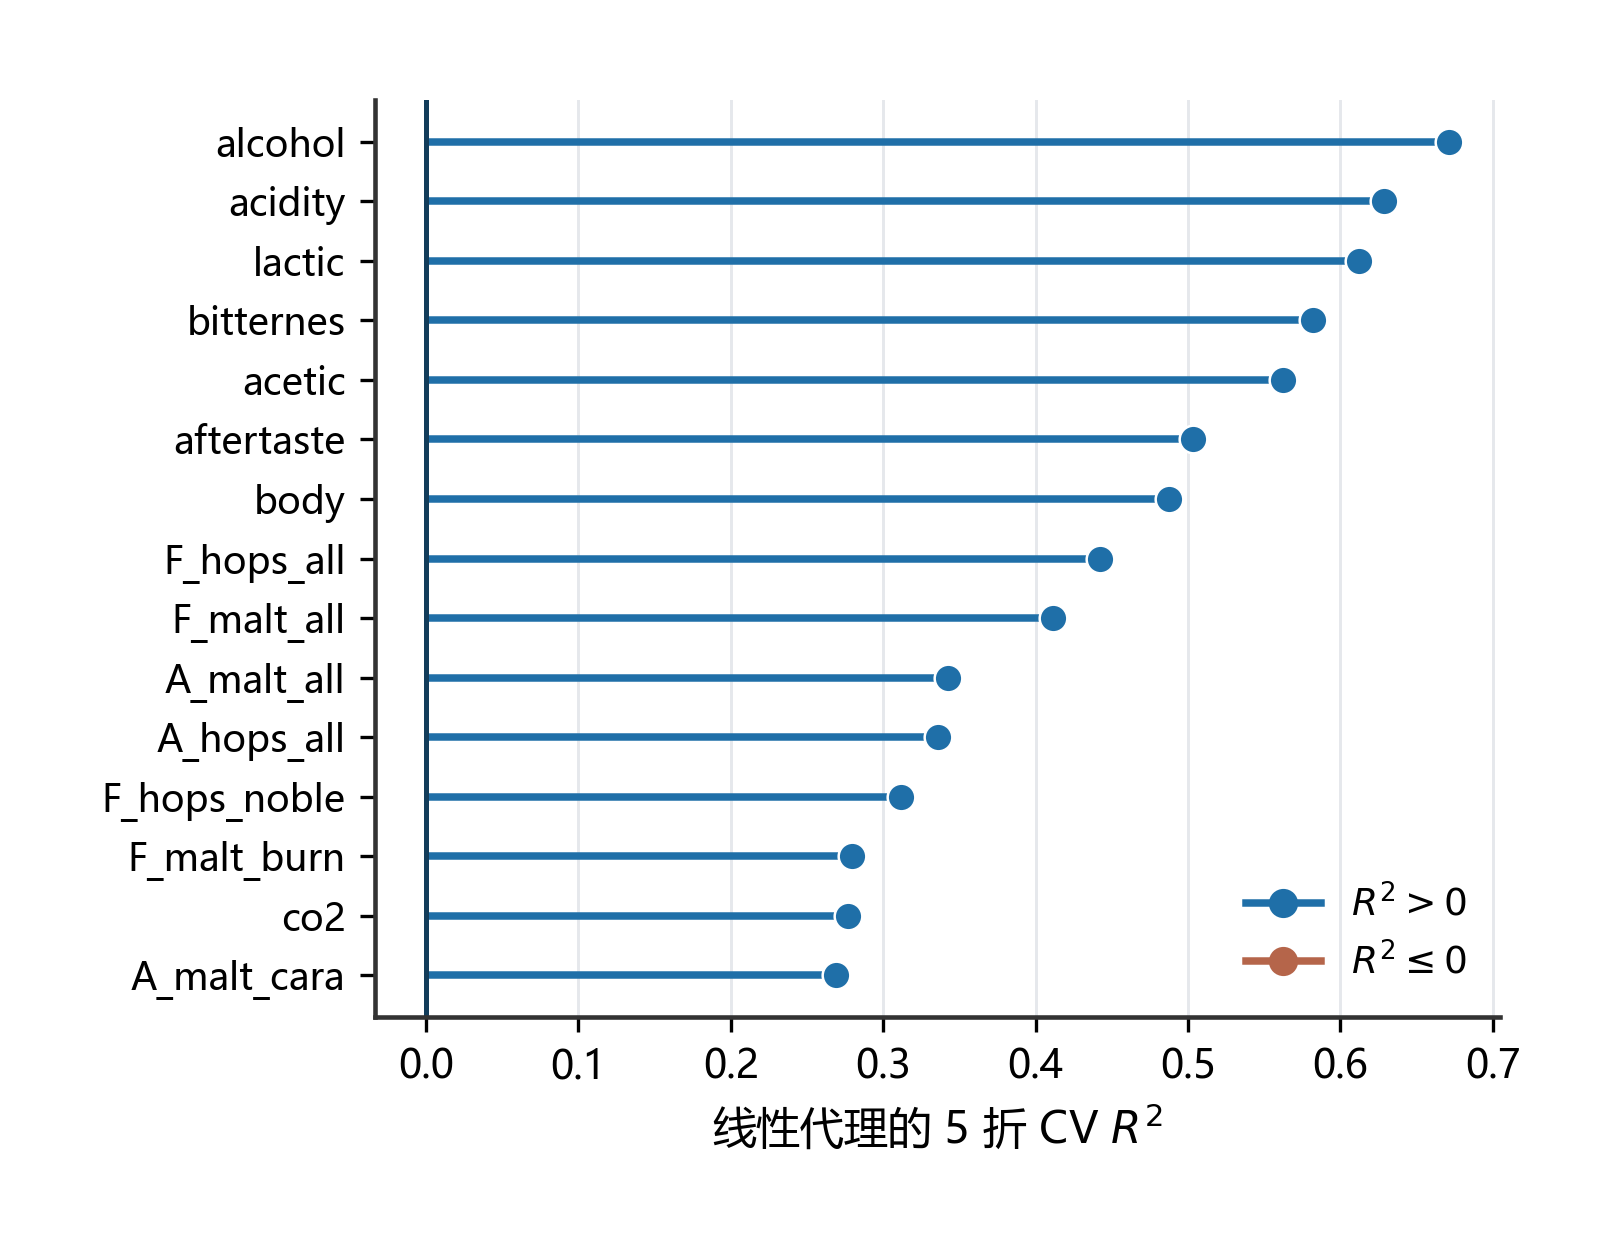
\includegraphics[width=\linewidth]{figures/fig_q3_surrogate_cv.png}
\caption{逐项交叉验证 $R^2$}
\label{fig:q3cvr2}
\end{subfigure}
\hfill
\begin{subfigure}[t]{0.48\textwidth}
\centering
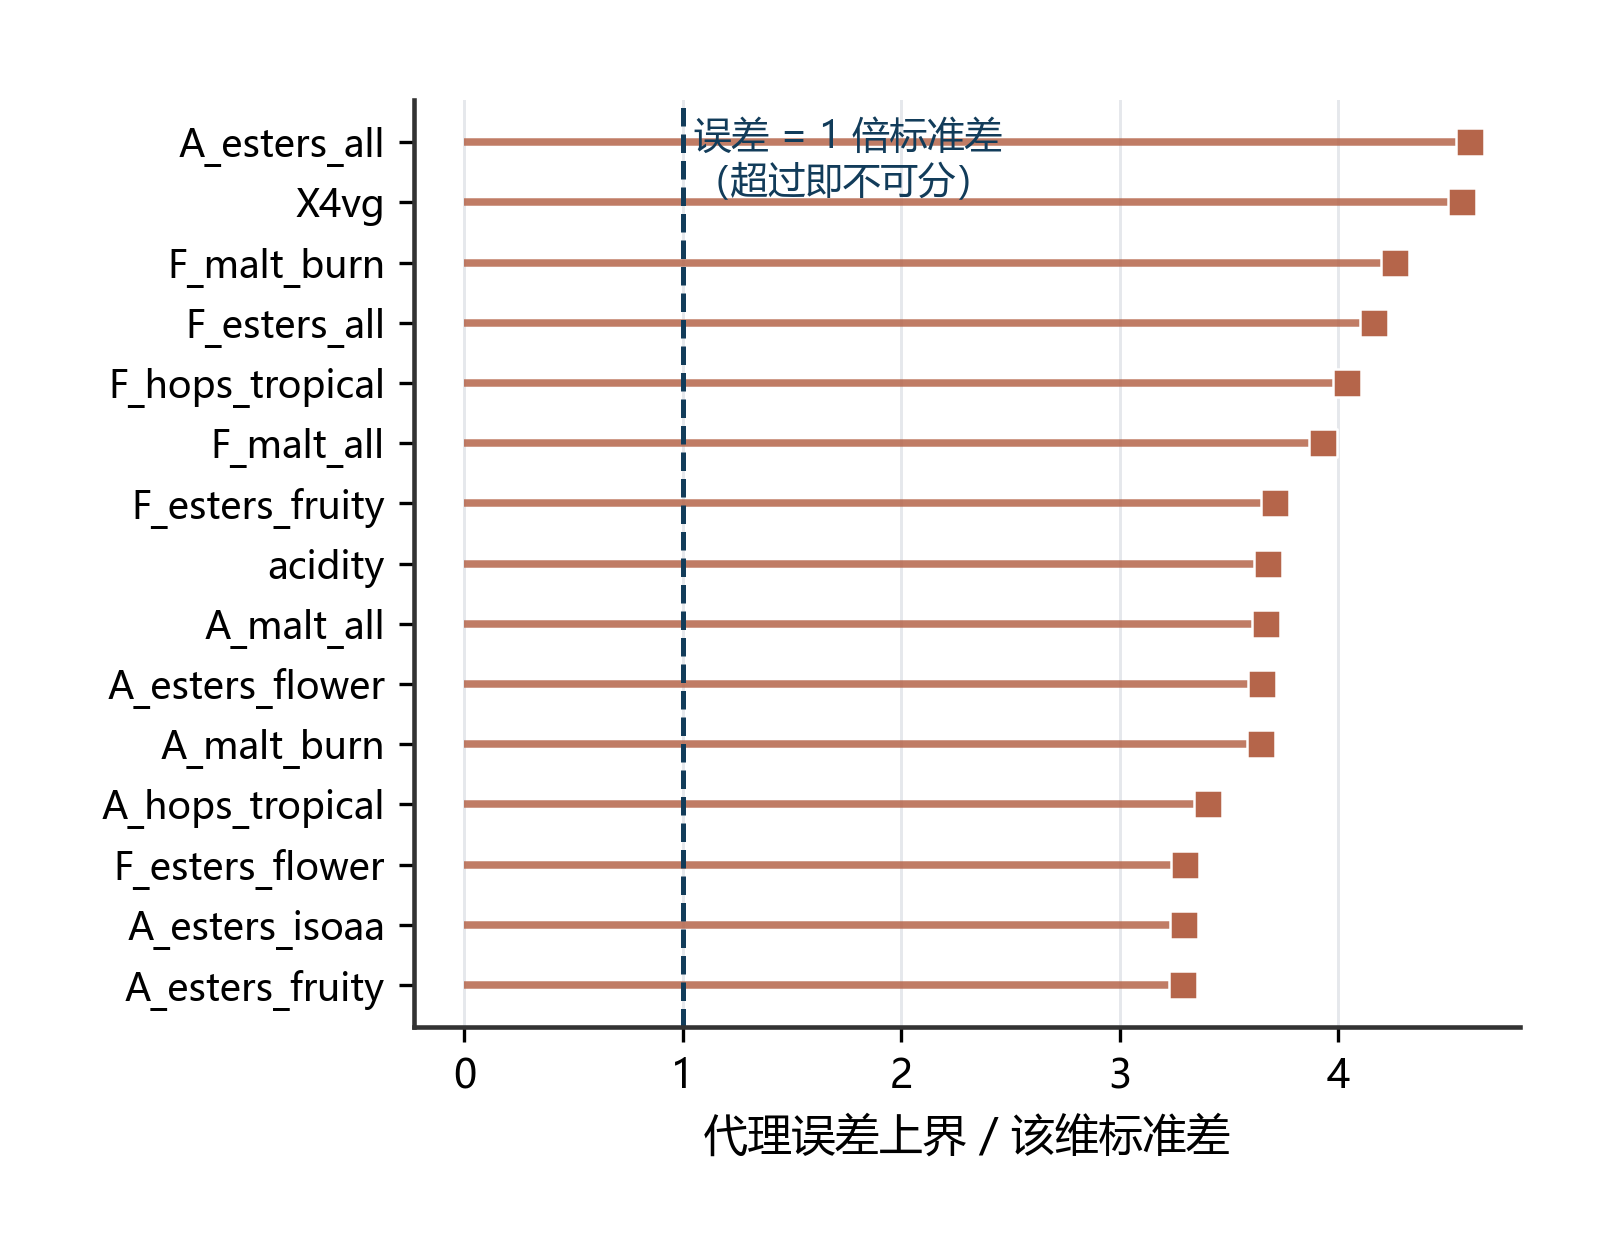
\includegraphics[width=\linewidth]{figures/fig_q3_surrogate_err.png}
\caption{误差与标准差之比}
\label{fig:q3err}
\end{subfigure}
\caption{感官代理的精度。左图为逐项 $R^2$，中位 0.1386；右图为误差与标准差之比，50 项的最大误差全部超过 1 倍标准差}
\end{figure}

两图合起来说明一件事：代理足以支撑“往哪个方向调”的判断，但不足以支撑“哪个点更好”的判断。这一结论在 8.4 节解释前沿可信边界时会直接用到。

\subsection{多目标混合整数线性规划}

以 $\log_{10}$ 域的浓度 $x_j$ 为决策变量，原始样本的浓度记为 $x_j^0$。三个目标定义为
\begin{align}
  f_1(x)&=\sum_{s=1}^{50}\frac{1}{\hat\sigma_s}\left|\hat y_s(x)-t_s\right|, \\
  f_2(x)&=\sum_{k\in\mathcal{K}}\max\left\{0,\ \frac{d_k(x)}{\tau_k}-1\right\}, \\
  f_3(x)&=\sum_{j\in\mathcal{J}}\left|x_j-x_j^0\right|,
\end{align}
$f_1$ 为按感官标准差加权的 $L_1$ 偏差，其中 $t_s$ 取目标风格内的中位感官值；$f_2$ 为缺陷物超阈值程度之和，$f_3$ 为干预代价。

约束分三类。硬约束要求 DMS 与 X4VG 不超阈值；软约束把双乙酰计入 $f_2$ 而不作硬限，因为其阈值在样本中位附近，硬压会与实际工艺相悖
\begin{equation}
  d_k(x)\le\tau_k,\quad k\in\{\text{DMS},\text{X4VG}\};\qquad
  d_{\text{diacetyl}}(x)\ \text{入}\ f_2 .
\end{equation}
改动量约束限制同时改动的化合物个数，以保证“定向重构”的工艺含义
\begin{equation}
  \sum_{j\in\mathcal{J}}z_j\le k_{\max}=25,\qquad
  \left|x_j-x_j^0\right|\le M_j z_j,\qquad z_j\in\{0,1\}.
\end{equation}
绝对值项经 $u_j\ge x_j-x_j^0$、$u_j\ge x_j^0-x_j$ 线性化，$f_1$ 中的 $|\hat y_s(x)-t_s|$ 同样拆成正负偏差变量。由此得到带 75 个 0--1 变量、326 个变量、406 条约束的混合整数线性规划，用 \emph{Gurobi 13.0.2} 求解。

三目标不可加权求和，因为 $f_1$、$f_2$、$f_3$ 的物理含义完全不同。本文用 $\varepsilon$-约束法：先分别解三个单目标得到支付表，再在 $f_2$、$f_3$ 的取值区间内取 $20\times15=300$ 个网格点，逐点求
\begin{equation}
  \min\ f_1(x)\quad \text{s.t.}\quad f_2(x)\le\varepsilon_2,\ f_3(x)\le\varepsilon_3,
\end{equation}
并加增广项剔除弱 Pareto 点。300 个网格点中 280 个可行，且这 280 点全部非支配，说明前沿的形状完全由目标之间的权衡决定，不是被可行性边界截断。

作为对照，本文手写 \emph{NSGA-II}：SBX 交叉 $\eta=15$、多项式变异 $\eta=20$，种群与代数按 75 维设定，在同样的缺陷物约束下得 115 个非支配点。

\subsection{模型求解}

\noindent\textbf{三个目标的无量纲化}\quad 三个目标的量级差别很大，直接加权会让感官偏差独占主导。因此先求理想点与最差点：单独最小化 $f_1$ 时得 $f_1=13.5064$、$f_2=87.1989$、$f_3=26.7886$；单独最小化 $f_2$ 时得 $f_1=48.7011$、$f_2=0$、$f_3=9.1529$；单独最小化 $f_3$ 时得 $f_1=47.2083$、$f_2=87.1989$、$f_3=1.0222$。由此得 $f_2$ 的极差为 87.1989、$f_3$ 的极差为 $26.7886-1.0222=25.7664$，归一化时按各自极差缩放。求理想点的 3 次求解中共有 20 个网格点不可行，为保持比较基准一致，理想点取在可行集内。

\noindent\textbf{ε-约束与网格}\quad 多目标按 ε-约束法处理：每次把 $f_2$、$f_3$ 各固定在一个水平上写成约束，只优化 $f_1$，遍历 $(f_2,f_3)$ 的 $20\times15=300$ 个组合。300 次求解中 280 次可行、20 次因硬约束冲突不可行，280 个可行点全部非支配，筛选后保留 5 个 Pareto 点。硬约束逐物取“阈值”与“基线”中更严的一条，即上限 $=\min(\log_{10}T_k,\,x_k^{0})$：DMS 的阈值换算值 1.2368 低于基线，故上限取 1.2368；4VG 的文献阈值 0.206\,mg/L 换算到对数域约 $-0.686$，但基线 $-2.0132$ 已低于该阈值，故取更严格的基线上限 $-2.0132$，该值不是阈值的对数换算值，软约束是双乙酰浓度不高于 0.2993，违约时以罚项 $\gamma=1.0$、权重 $\lambda=0.1$ 计入 $f_1$。

\noindent\textbf{求解规模与耗时}\quad 每个网格点对应一个混合整数线性规划：326 个变量（其中 75 个 0--1、251 个连续）、406 条约束，其中感官代理的 50 条线性等式由 8 成分偏最小二乘回归给出。求解器用 Gurobi，采用默认的自动算法选择，对偶单纯形与内点法按规模自动切换，300 个网格点串行求解总耗时 47.7 秒，单点平均 0.159 秒。这个速度使得 280 个点的全网格遍历比启发式搜索更划算，也解释了为什么本文没有采用 NSGA-II 作为主方案。

\noindent\textbf{结果的核验}\quad 生成是否退化为复制，用最近邻距离检验：生成谱到真实样本的最近邻距离中位 13.6019，真实样本彼此的最近邻距离中位 12.6409，比值 1.076，说明生成谱既未落进训练集的凸包内部，也没有外推到远离数据的高风险区域。前沿是否真的更优，用 NSGA-II 在相同约束下独立跑出的 115 个非支配点作对照：本文的 5 个精确点支配其中 105 个（91.30\%），反向支配为 0，超体积 688.54 对 299.12。

\subsection{结果分析}

5 个 Pareto 点全部为 OPTIMAL 状态，$mip\_gap=0$，两两互不支配，见表~\ref{tab:q3}。硬约束的超出量取 $t_k-\tau_k$，负值即低于阈值，在五点上的最小值为 $-0.644$(P4)，即最贴近阈值的那条约束仍留有余量。基线感官偏差为 48.9620，最优解 23.8519，降幅 51.3\%。

\begin{table}[htbp]
\centering
\footnotesize
\caption{问题三的 Pareto 前沿，以 Tripel 为目标风格}
\label{tab:q3}
\begin{minipage}{\textwidth}\footnotesize
注：五个点的 $f_2$ 均为 0.0000，缺陷维度在本例中不活跃，前沿实际是 $f_1$--$f_3$ 的二维权衡，$f_2$ 只作可行性校验。
\end{minipage}
\begin{tabular*}{\textwidth}{@{\extracolsep{\fill}}ccccc@{}}
\toprule
\textbf{点} & $f_1$（感官偏差） & $f_2$（缺陷风险） & $f_3$（改动代价） & \textbf{改动化合物数} \\
\midrule
P1 & 23.8519 & 0.0000 & 7.4510 & 7 \\
P2 & 25.2188 & 0.0000 & 6.4250 & 6 \\
P3 & 27.1161 & 0.0000 & 5.3507 & 5 \\
P4 & 30.3666 & 0.0000 & 4.2891 & 4 \\
P5 & 37.3603 & 0.0000 & 2.1439 & 2 \\
\bottomrule
\end{tabular*}
\end{table}

这里要记录一处必要的单位处理。缺陷物阈值必须换算到各列在附件1 中的实际量纲域：DMS 与 4VG 在 $\log_{10}$ 域，双乙酰与 trans-2-壬烯醛在 mg/L 线性域(依据 5.3 节的逐列标记，并经附件8 的 Calibrated 表交叉验证)。若一律取 $\log_{10}$，线性域列的软约束会退化为与决策无关的常数，$f_2$ 被固定而失去意义。修正后 $f_2$ 能真正降到 0，这一变化本身就是“约束是否在起作用”的检验。

五个点的改动数单调递减：P1 改动乙醛、DMS、异戊酸乙酯、苯乙醛、异丁酸异戊烯酯、松油烯-4-醇与苯乙酸乙酯共 7 个；P2 去掉苯乙酸乙酯；P3 再去掉异戊酸乙酯，剩 5 个；P4 去掉松油烯-4-醇，剩 4 个；P5 换了一套组合，只改 DMS 与甲基吡嗪 2 个。前四点的改动集合逐级包含，说明前沿是从同一组化合物里逐步削减而成；第五点换了另一条路线，用最小干预换取可接受的偏差。真正被调动的化合物始终不出这 8 个，其余 67 个决策变量被阈值与改动上限卡住——这是一条可解释的结论：在给定阈值下能有效调节风味指纹的化合物是少数。

从改动方向看，见图~\ref{fig:q3opt}；DMS 在所有点上都被下调，从 1.587 压到 0.593 至 1.237 之间，取 $\log_{10}$ 域，阈值为 1.237；松油烯-4-醇从 5.222 直接降到检出限 $-1.818$，异戊酸乙酯从 $-2.390$ 降到 $-4.487$，乙醛从 0.808 降到 $-0.464$ 至 $-0.745$，异丁酸异戊烯酯从 5.169 降到 0.823。唯一上调的是苯乙醛，从 0.021 升到 0.238。DMS 是熟蔬菜味缺陷物，下调符合目标风格；松油烯-4-醇带木香与松节油气息，在 Tripel 的高酯香型中属可牺牲项；苯乙醛上调与 Tripel 的蜂蜜甜香一致。方向在酿造学上自洽，说明约束与代理没有把结果推向化学上荒谬的解。

\begin{figure}[htbp]
\centering
\begin{subfigure}[t]{0.48\textwidth}
\centering
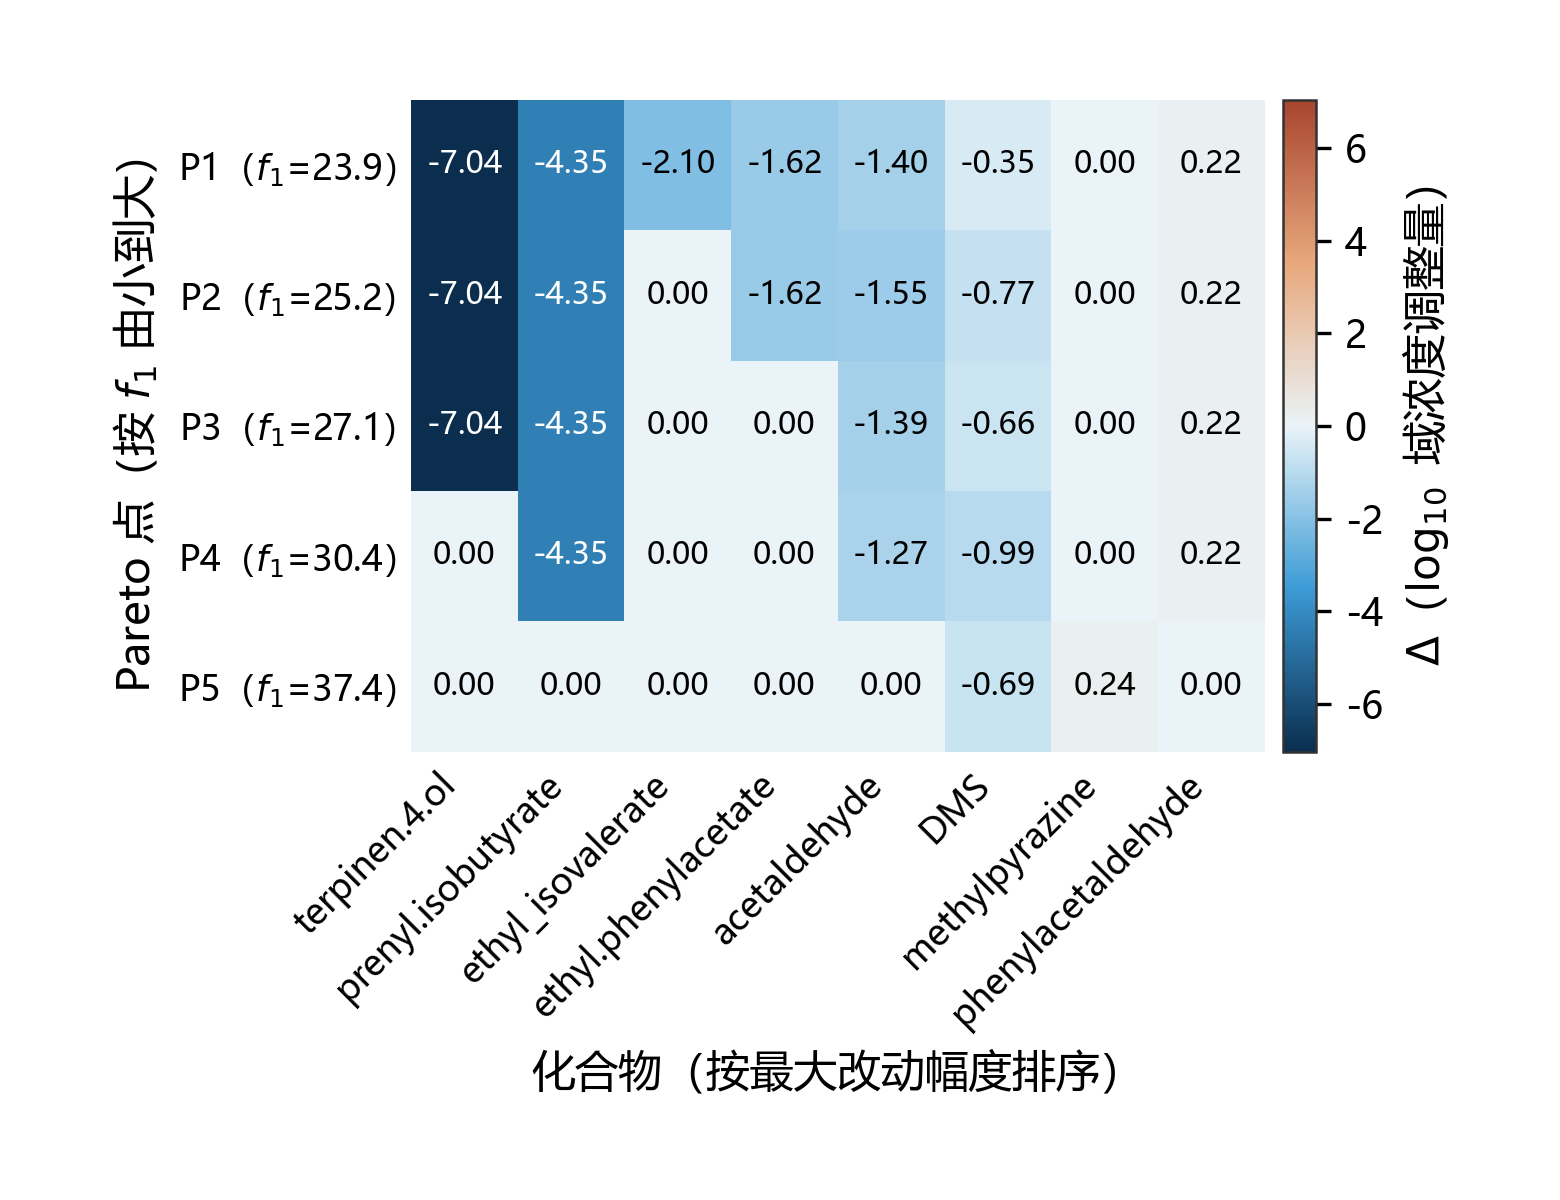
\includegraphics[width=\linewidth]{figures/fig_q3_deltas.png}
\caption{改动化合物与幅度}
\end{subfigure}
\hfill
\begin{subfigure}[t]{0.48\textwidth}
\centering
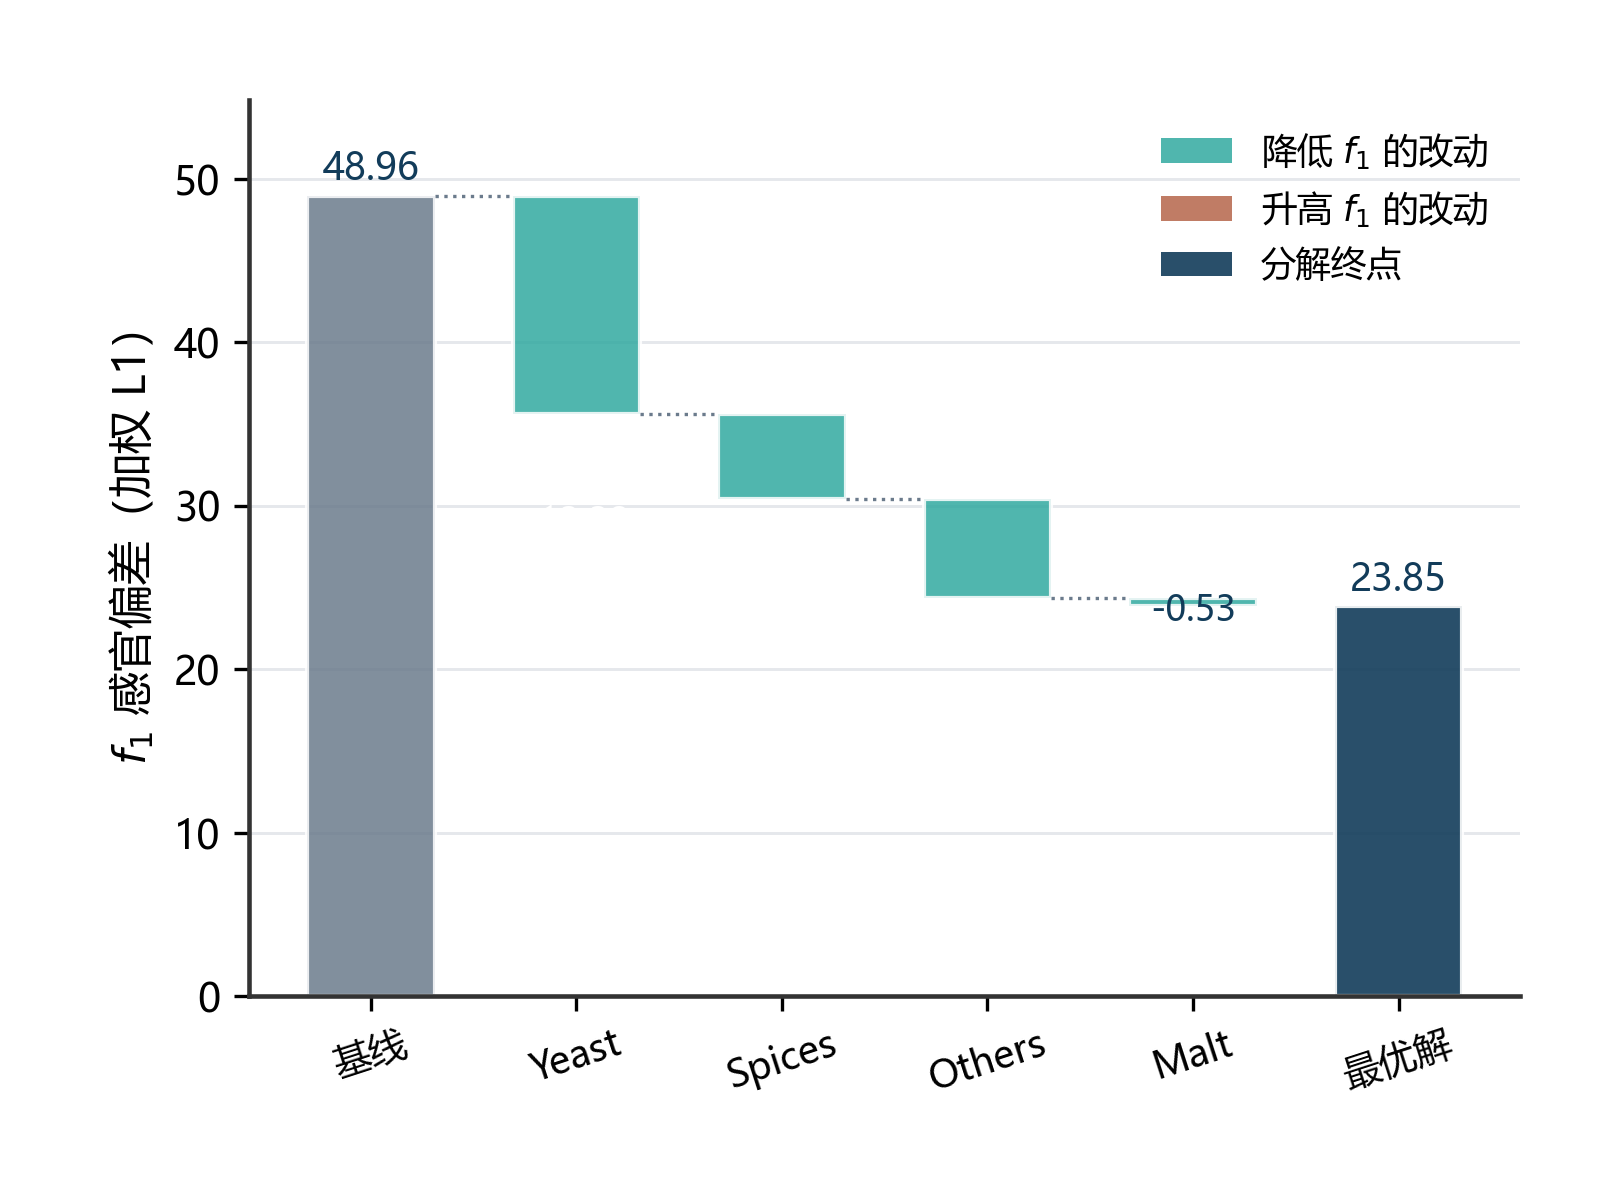
\includegraphics[width=\linewidth]{figures/fig_q3_waterfall.png}
\caption{$f_1$ 的逐组分解}
\end{subfigure}
\caption{最优解改了什么。左图为 8 个化合物的调整幅度，DMS 与松油烯-4-醇下调最重；右图为 $f_1$ 的逐组分解，降幅主要来自酸度、苦度与硫味三类}
\label{fig:q3opt}
\end{figure}

精确解与启发式的对比是本章的第二个结论。5 个精确点支配了 115 个 NSGA-II 点中的 91.30\%，反向支配比例为 0；超体积 688.54 对 299.12，增益 389.42(图~\ref{fig:q3front})。这为“以精确混合整数规划为主、启发式为对照”的路线提供了机械证据。

\begin{figure}[htbp]
\centering
\begin{subfigure}[t]{0.48\textwidth}
\centering
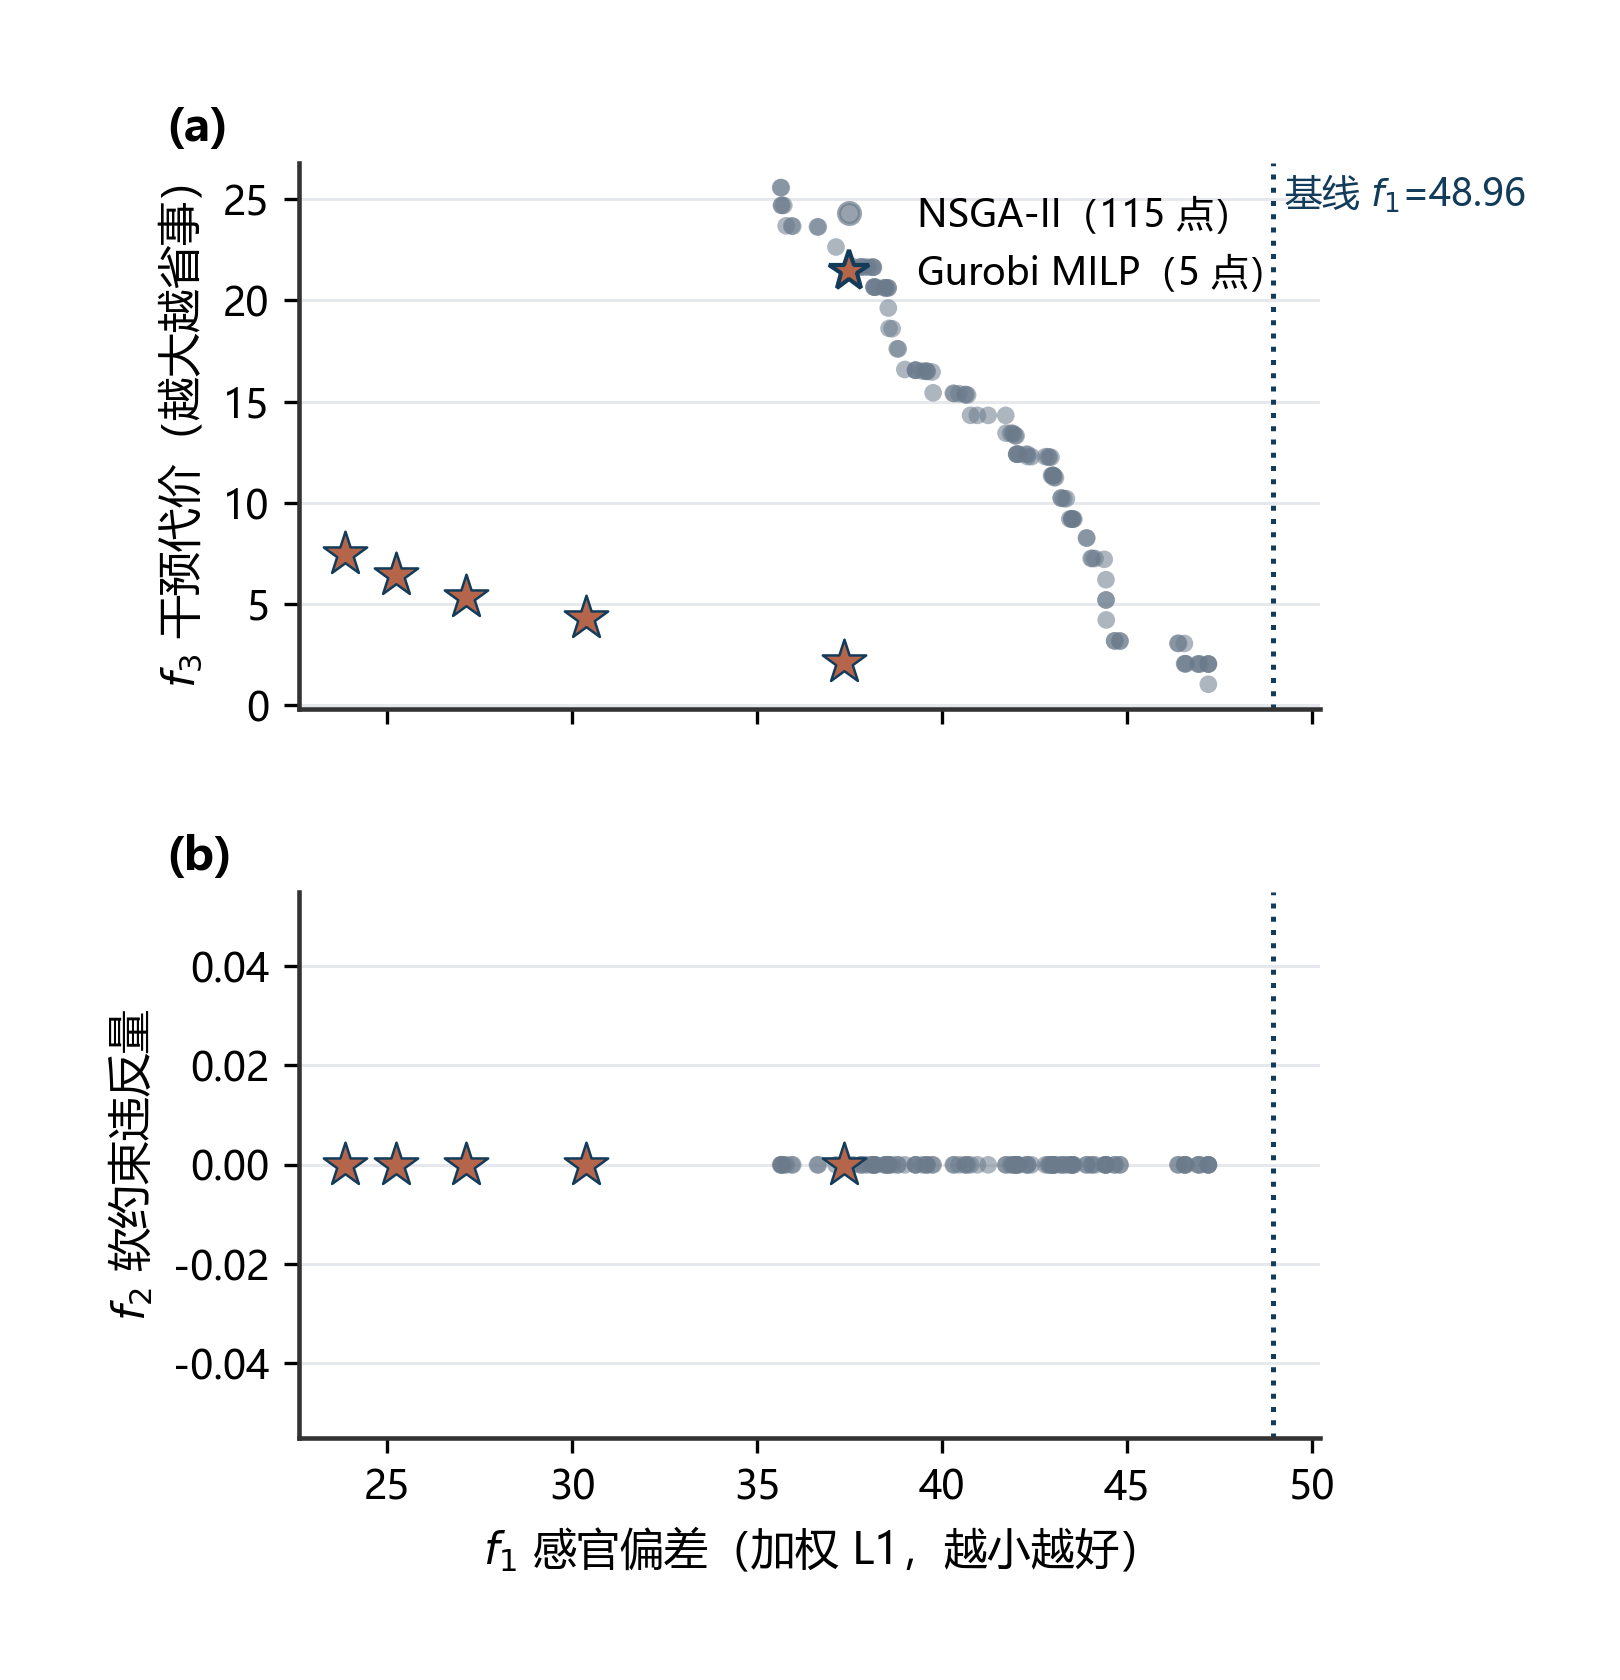
\includegraphics[width=\linewidth]{figures/fig_q3_front.png}
\caption{混合整数规划前沿与 NSGA-II 前沿的双投影对比：精确前沿整体位于启发式前沿的左下方}
\label{fig:q3front}
\end{subfigure}
\hfill
\begin{subfigure}[t]{0.48\textwidth}
\centering
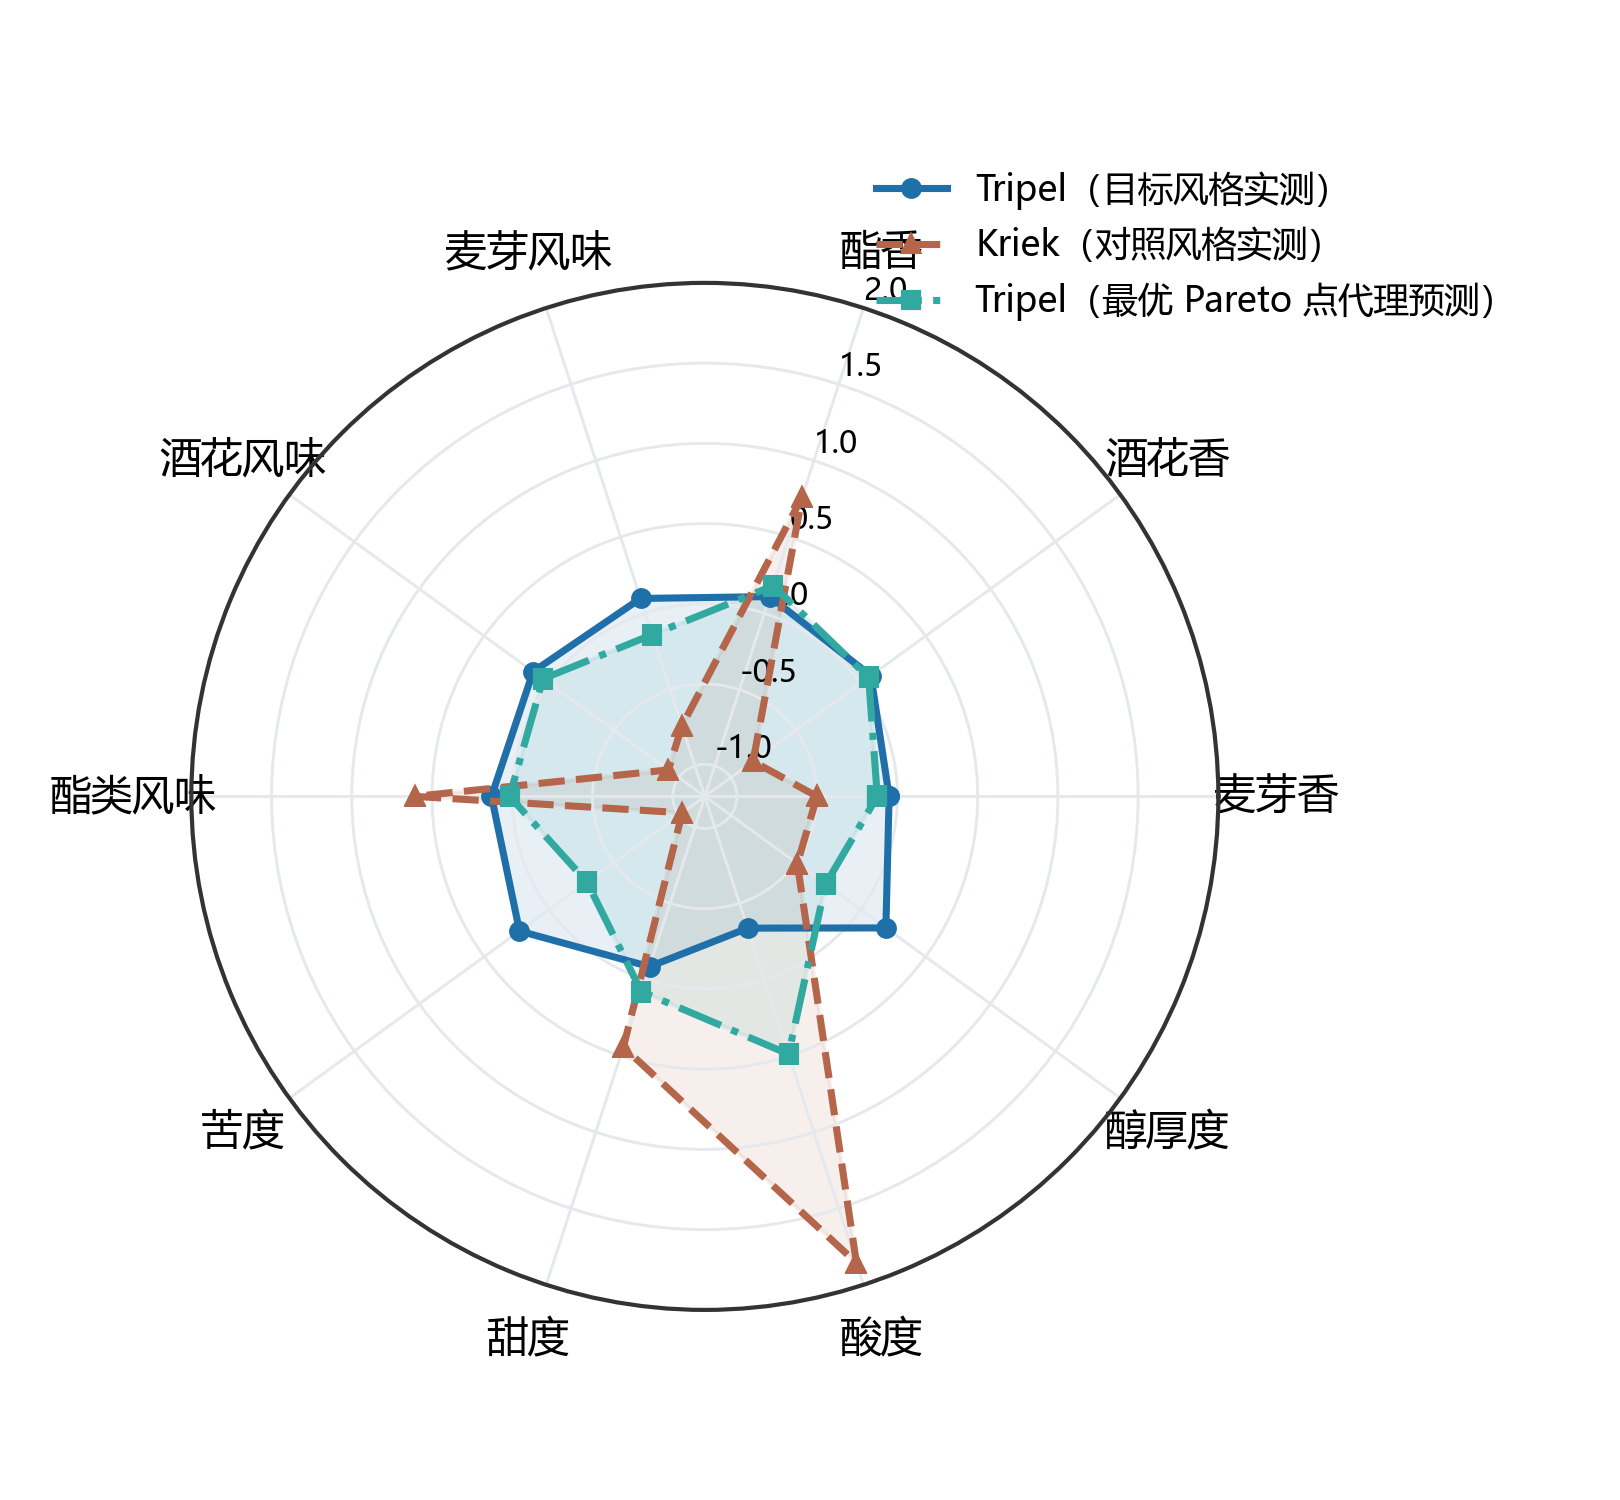
\includegraphics[width=\linewidth]{figures/fig_q3_radar.png}
\caption{目标风格、对照风格与最优解的感官画像：最优解在气味维度贴近 Tripel，在口感维度偏向 Kriek}
\label{fig:q3radar}
\end{subfigure}
\caption{前沿与画像。左图为混合整数规划前沿与 NSGA-II 前沿的双投影对比，精确前沿整体位于启发式前沿的左下方；右图为目标风格、对照风格与最优解的感官画像}
\end{figure}

第三个结论关系结果的可信边界。五点之间的 $f_1$ 间隙依次为 1.3669、1.8973、3.2505、6.9936，而代理误差中位 0.4626、95\% 分位 1.4124、上界 3.1525。P1 与 P2 的间距小于 95\% 分位误差，统计上不可分；P2 与 P3 略大于分位误差但仍小于上界，只能算弱可分；后两个间隙大于上界，可以分辨。因此本文把前沿报成三段(P1--P2、P3、P4--P5)，段内不作排序，也不指定唯一最优解。

图~\ref{fig:q3radar} 与表~\ref{tab:q3profile} 给出感官画像。气味描述类基本贴合目标：酒花香的嗅觉维度由 0.079 到 0.061、酯香的嗅觉维度由 0.109 到 0.180、苦度由 0.228 到 $-0.292$；口感类偏离较多：麦芽香的嗅觉维度由 $-0.052$ 到 $-0.125$、麦芽香的风味维度由 0.097 到 $-0.140$、酒体由 0.194 到 $-0.270$、酸度由 $-0.337$ 到 0.489。



\begin{table}[htbp]
\centering
\footnotesize
\caption{三个风格画像在 10 个感官项上的取值，按附件4 连续强度尺度，末列为最优解相对目标的偏差}
\label{tab:q3profile}
\begin{tabular*}{\textwidth}{@{\extracolsep{\fill}}lcccc@{}}
\toprule
\textbf{感官项} & \textbf{Tripel 实测} & \textbf{Kriek 实测} & \textbf{最优解预测} & \textbf{偏差} \\
\midrule
麦芽香（嗅觉） & -0.051 & -0.501 & -0.125 & -0.074 \\
酒花香（嗅觉） & 0.079 & -0.828 & 0.061 & -0.018 \\
酯香（嗅觉） & 0.109 & 0.762 & 0.180 & +0.071 \\
麦芽香（风味） & 0.097 & -0.738 & -0.140 & -0.237 \\
酒花香（风味） & 0.123 & -0.919 & 0.047 & -0.076 \\
酯香（风味） & 0.130 & 0.605 & 0.017 & -0.113 \\
苦度 & 0.228 & -1.026 & -0.292 & -0.520 \\
甜度 & -0.084 & 0.443 & 0.079 & +0.164 \\
酸度 & -0.337 & 1.856 & 0.489 & +0.826 \\
酒体 & 0.194 & -0.488 & -0.270 & -0.464 \\
\bottomrule
\end{tabular*}
\end{table}

麦芽香与酒体偏离最大，原因不在优化方向，而在决策列的构成。75 维决策列由问题二的香气类 Top-3 并集构成，而酒体的化学载体乙醇、麦芽香的载体色度 EBC 都属于理化指标，按问题二的处理方式被排除在香气化合物之外，因而不在决策列内，优化无法直接调节它们。这两项的预测变化全部来自偏最小二乘代理把香气列改动的线性外推——这既是 $f_1$ 只能降到 23.8519 而无法归零的原因，也说明在“只改香气化合物”的工艺前提下，口感项的改进必须另找手段。

\subsection{跨风格迁移}

题面还要求做跨风格迁移：把某一风格的化合物谱迁移为目标风格，同时保持缺陷化合物不恶化。本文取源风格 Pils/Lager(11 个样本)、目标风格 Tripel(28 个样本)，把源风格化学谱的中位数作为被迁移的起点 $x^0$，目标感官谱取 Tripel 中位数，其余设定与上一节一致(决策列 75 维、偏最小二乘代理、$\varepsilon$-约束)。

本节对缺陷物的处理更严格，因为迁移场景下“不恶化”是硬要求。五类缺陷物的约束方式如下：DMS 与 4VG 硬约束到 $\min(\theta,x^0)$；双乙酰除硬约束到 $\min(\theta,x^0)$ 外，超阈部分仍计入 $f_2$;trans-2-壬烯醛按文献阈值 0.11 $\mu$g/L 处理——附件8 该行的阈值单元格为 NA，只给了列名与单位，因此必须外部引用，不能声称取自附件；Stale hops 不是化合物而是感官描述项，用代理模型约束其预测值不超过迁移前的预测值。各类缺陷物在迁移前后的取值见表~\ref{tab:q3transfer}。

\begin{table}[htbp]
\centering
\footnotesize
\caption{跨风格迁移 Pils/Lager $\to$ Tripel 的缺陷物控制}
\label{tab:q3transfer}
\begin{tabular*}{\textwidth}{@{\extracolsep{\fill}}llccc@{}}
\toprule
\textbf{缺陷物} & \textbf{阈值来源} & \textbf{迁移前} & \textbf{迁移后} & \textbf{是否恶化} \\
\midrule
DMS & 附件8，17.25 $\mu$g/L & 1.1793 & 1.1793 & 否 \\
Diacetyl & 附件8，0.299 mg/L & 0.0570 & 0.0570 & 否 \\
4VG & 附件8，0.206 mg/L & $-2.0132$ & $-2.0132$ & 否 \\
trans-2-nonenal & 文献，0.11 $\mu$g/L & 0.002012 & 0.002012 & 否 \\
Stale hops & 代理预测（感官项） & 0.2528 & 0.0453 & 否（改善） \\
\bottomrule
\end{tabular*}
\end{table}

五类缺陷物全部满足不恶化：DMS、双乙酰、4VG 在迁移前就已低于或等于阈值，trans-2-壬烯醛保持不变，Stale hops 的代理预测从 0.2528 降到 0.0453，是唯一明显改善的一项。这里要指出一处数据本身的限制：按附件8 标注的 mg/L 单位换算，文献阈值 0.11 $\mu$g/L 折合 $1.1\times10^{-4}$ mg/L，低于该列在样本中的 1\% 分位($1.61\times10^{-4}$)，即数据集内没有任何样本满足该阈值。这种情况下“不超标”不可达，本文只保证“不恶化”，并如实记录这一单位上的存疑。

迁移的效果是感官偏差从起点 $x^0$ 的 47.1450 降到 13.1366，降幅 72.14\%，改动了 25 个化合物(正好等于干预预算上限)。同时验证了缺陷硬约束的代价：若撤掉缺陷上界，$f_1$ 仍是 13.1366，即“不恶化”在本次迁移中没有付出额外代价。

这个 72.14\% 明显高于上一节的 51.3\%，原因是起点不同：上一节从 Tripel 自身中位数出发，本节从 Pils/Lager 的化学谱出发，后者离目标远得多，可改进空间也大。两条路线的降幅不可直接比较，报告时必须同时给出起点与起点处的偏差。

以上结果都是化学谱层面的设计候选。代理模型未经真实感官实验校验，优化不含化合物间的协同与拮抗，只能作为配方调整的方向性建议。

\subsection{灵敏度分析}

前沿位置依赖六个设定：干预预算 $k_{\max}$、改动列代价 $\gamma$、改动量代价 $\lambda$、缺陷容忍 $\varepsilon_2$、工艺预算 $\varepsilon_3$ 与代理成分数。本文对每个参数做单因素扰动，每次扰动都重新求解一次混合整数规划，共 27 次重解，以最优 $f_1$ 的变化为响应。基准设定 $\gamma=1$、$\lambda=0.1$、$k_{\max}=25$，此处 $f_1=13.7852$。结果见表~\ref{tab:q3sens} 与图~\ref{fig:q3tornado}。

\begin{table}[htbp]
\centering
\footnotesize
\caption{问题三灵敏度分析，基准 $f_1=13.7852$}
\label{tab:q3sens}
\begin{tabular*}{\textwidth}{@{\extracolsep{\fill}}lcccc@{}}
\toprule
\textbf{参数} & \textbf{扰动范围} & \textbf{$f_1$ 范围} & \textbf{摆幅} & \textbf{改动化合物数} \\
\midrule
改动列代价 $\gamma$ & $[0.5,\ 4.0]$ & $[11.080,\ 24.424]$ & 13.3438 & 10 $\to$ 1 \\
代理成分数 & $[4,\ 13]$ & $[20.244,\ 29.475]$ & 9.2310 & 5 $\to$ 7 \\
工艺预算 $\varepsilon_3$ & $[4.47,\ 11.92]$ & $[11.156,\ 17.061]$ & 5.9057 & 3 $\to$ 9 \\
改动量代价 $\lambda$ & $[0.05,\ 0.40]$ & $[12.670,\ 17.217]$ & 4.5471 & 6 $\to$ 5 \\
缺陷容忍 $\varepsilon_2$ & $[0.0005,\ 0.002]$ & 13.785（恒定） & 0.0000 & 6 $\to$ 6 \\
干预预算 $k_{\max}$ & $[15,\ 35]$ & 13.785（恒定） & 0.0000 & 6 $\to$ 6 \\
\bottomrule
\end{tabular*}
\end{table}

\begin{figure}[htbp]
\centering
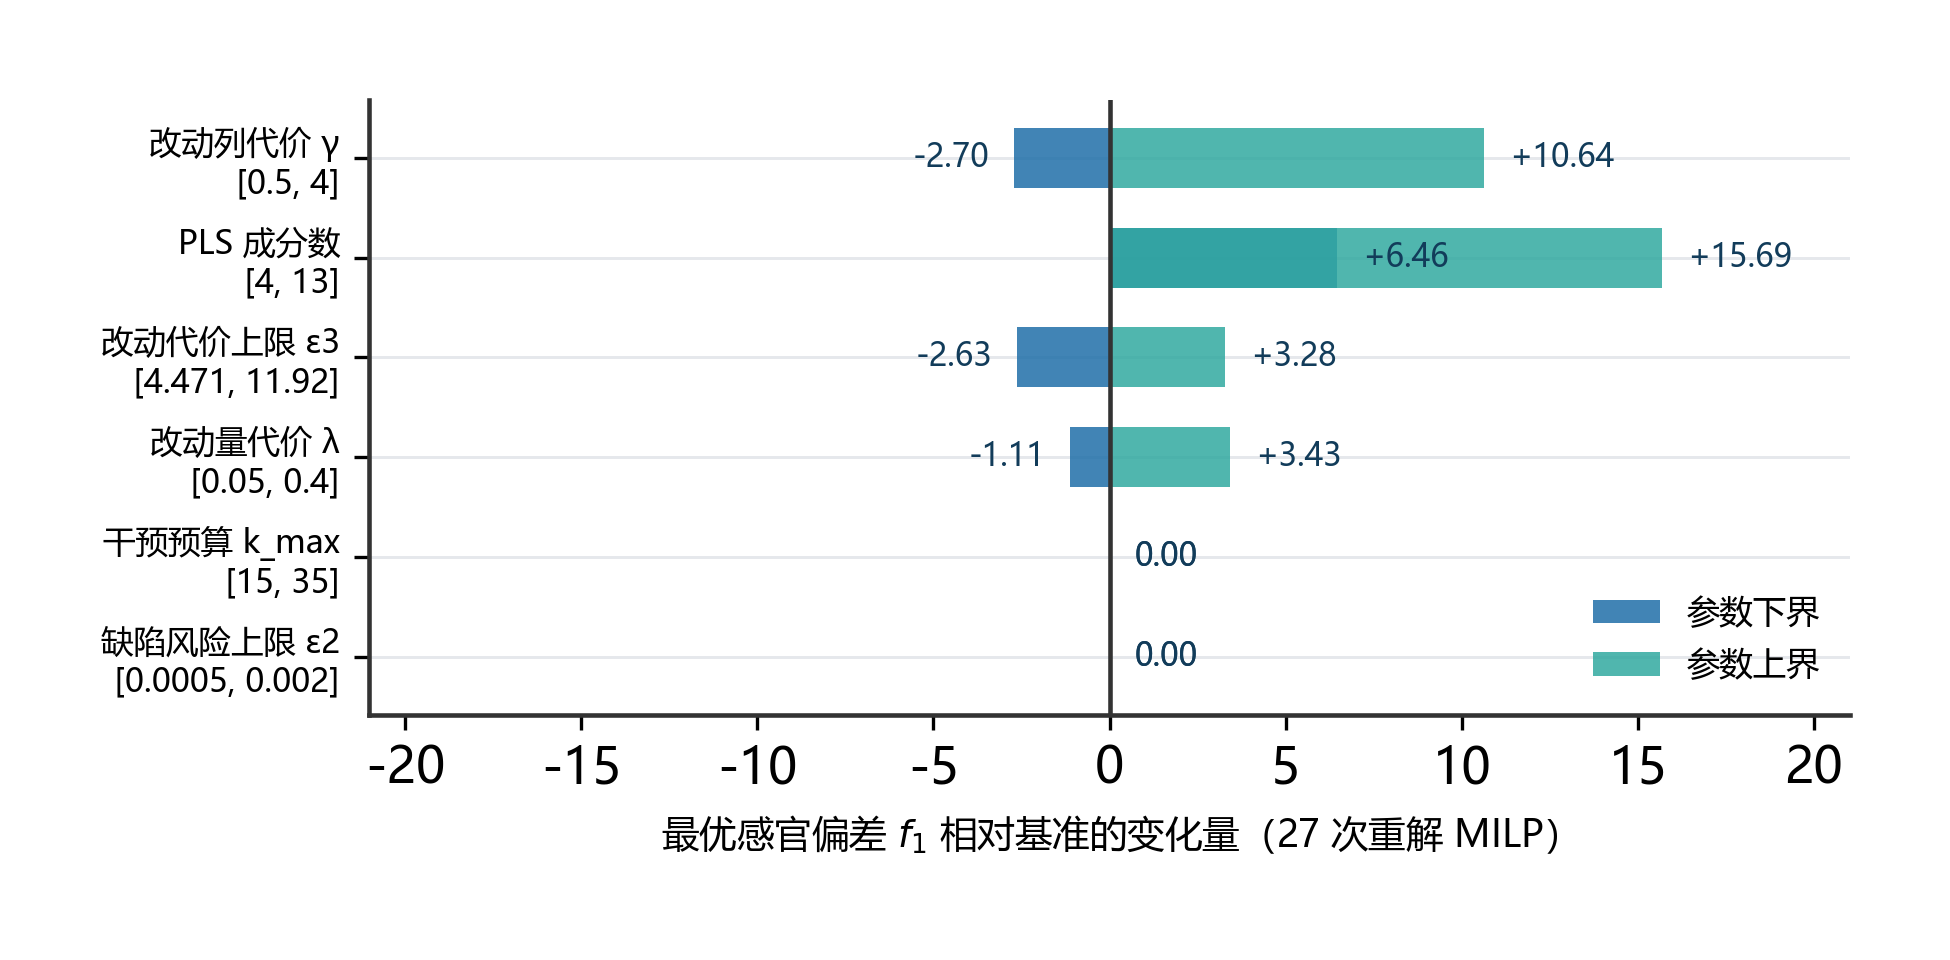
\includegraphics[width=0.79\textwidth]{figures/fig_q3_tornado.png}
\caption{灵敏度分析：27 次重解得到的 $f_1$ 变化量，$\gamma$ 与代理成分数是主导项}
\label{fig:q3tornado}
\end{figure}

三条结论。第一，改动列代价 $\gamma$ 是主导项，摆幅 13.3438，远大于其余各项。$\gamma$ 增大使同一 $\varepsilon_3$ 预算下可改的列数从 10 降到 1,$f_1$ 从 11.080 升到 24.424。这说明“愿意改几个化合物”对结果的影响大于任何数值细节，本文因此把改动数作为显式约束。

第二，代理成分数是第二敏感项，摆幅 9.2310，且不单调：取 4 个成分时 $f_1=25.675$(拟合不足),6 个时降到 20.244,8 个为 20.576，增加到 13 个反而升到 29.475。摆幅超过 9 意味着代理的复杂度设定本身就能让前沿移动三成以上，这是本文坚持“只按段报告、不报单点最优”的量化依据。

第三，缺陷容忍 $\varepsilon_2$ 与干预预算 $k_{\max}$ 的摆幅均为 0，在本例中都是不活跃约束。$\varepsilon_2$ 不活跃是因为双乙酰已被硬约束压到阈值以下，此时 $f_2=0$，放宽上限自然无影响——这正是单位修正后的结果，修正前 $f_2$ 被伪约束固定，扰动 $\varepsilon_2$ 会看似敏感。$k_{\max}$ 不活跃是因为最优解只需改 6 个化合物，上限从 15 放宽到 35 都不变。两点都须写明，否则容易把 $k_{\max}=25$ 误当作结论的驱动因素。
